\chapter{الإنزيمات والحفز الكيميائي الحيوي}\label{ch:b1:enzymes}

صبّ ماءً أكسجينيًا على بطاطا مقطوعة فترغي: إذ يشطر جزيء واحد من
الكاتالاز في \omterm{def:b1:cell-unit-of-life:cell}{خلايا} البطاطا أربعين مليون جزيء من الماء الأكسجيني في كل
ثانية، وهو تفاعل كان ليستغرق سنين لو تُرك لنفسه. والماء الأكسجيني كان
سيتفكك على كل حال --- فالتفاعل هبوطي --- لكن لا في زمن نافع. وكل
تفاعل في \omterm{def:b1:cell-unit-of-life:cell}{الخلية} كهذا: فالترموديناميك يقول إلى أي جهة يستطيع أن يجري،
و\emph{\omterm{def:b1:enzymes:enzyme}{الإنزيم}} يقول هل يجري الآن. يصف هذا الفصل ما يفعله \omterm{def:b1:enzymes:enzyme}{الإنزيم}
بتفاعل، والحركية التي تُقاس بها \omterm{def:b1:enzymes:enzyme}{الإنزيمات} وتُقارن، وطرق تثبيطها،
وطرق تشغيل \omterm{def:b1:cell-unit-of-life:cell}{الخلية} لها وإطفائها.

\section{الحفز}

\begin{definition}[الإنزيم والركيزة والموقع الفعال]\label{def:b1:enzymes:enzyme}
\emph{الإنزيم}\index{إنزيم} \omterm{def:b1:proteins:peptide}{بروتين} (ونادرًا \omterm{def:b1:nucleic-acids:chain}{RNA}) \emph{يحفّز}
تفاعلًا: أي يزيد معدله دون أن يُستهلك ودون أن يغير التوازن.
والجزيئات التي يعمل عليها \emph{ركائزه}\index{ركيزة}؛ وهي ترتبط في
\emph{الموقع الفعال}\index{الموقع الفعال}، وهو شق تبطنه بضع بقايا،
وفيه تجري الكيمياء. والإنزيمات \emph{نوعية} --- لركيزة واحدة أو
لعائلة، ولرابطة واحدة، ولمصاوغ فراغي واحد --- وتُسمى بركيزتها
وتفاعلها باللاحقة \emph{-از} (اللاكتاز، وبوليميراز \omterm{def:b1:nucleic-acids:chain}{DNA}، ونازعة
هيدروجين السكسينات)، في ستة أصناف: المؤكسدات المرجعة، والناقلات،
والحالّات المائية، والفالقات، والمصاوغات، والرابطات. وكثير منها يحتاج
إلى \emph{عامل مرافق}\index{عامل مرافق} غير بروتيني: شاردة معدنية
(Zn، وMg، وFe)، أو \emph{مرافق إنزيمي}\index{مرافق إنزيمي} عضوي ---
$\mathrm{NAD^+}$، وFAD، \omterm{def:b1:water-small-molecules:ph}{والمرافق} A، ومعظمها مصنوع من فيتامينات، وهذا
هو ما تفيده الفيتامينات.
\end{definition}

\begin{proposition}[ما يغيره الإنزيم وما لا يغيره]\label{prop:b1:enzymes:whatitdoes}
\index{طاقة التنشيط}\index{الحالة الانتقالية}
يمر التفاعل \emph{بحالة انتقالية}، وهي ترتيب مجهد للذرات أعلى طاقةً
حرة من المتفاعلات والنواتج بمقدار \emph{\omterm{prop:b1:enzymes:whatitdoes}{طاقة التنشيط}} $E_a$؛ ولا
يتفاعل إلا ما يحمله الاضطراب الحراري فوق هذا الحاجز من جزيئات، بكسر
يتناسب مع $e^{-E_a/RT}$. \omterm{def:b1:enzymes:enzyme}{والإنزيم} يرتبط \omterm{prop:b1:enzymes:whatitdoes}{بالحالة الانتقالية} ارتباطًا
أوثق من ارتباطه بالركيزة --- إذ يكون موقعه الفعال متكاملًا مع الصورة
المجهدة --- فيخفض $E_a$: وخفضها بمقدار \qty{34}{kJ/mol} (وهي قيمة
بضع \omterm{def:b1:water-small-molecules:water}{روابط هيدروجينية}) عند \qty{37}{\celsius} يضرب المعدل في
$e^{34\,000/2580} \approx
10^6$. وهو لا يغير $\Delta G$ ولا ثابت
التوازن، وهما لا يتوقفان إلا على المتفاعلات والنواتج: \omterm{def:b1:enzymes:enzyme}{فالإنزيم} يسرّع
التفاعلين الأمامي والخلفي بالقدر نفسه ويبلغ بالجملة التوازن نفسه أسرع.
\end{proposition}

\begin{omfigure}
\begin{tikzpicture}
\begin{axis}[
  width=0.86\linewidth, height=6.2cm,
  axis x line=bottom, axis y line=left,
  xmin=0, xmax=10, ymin=0, ymax=10,
  xlabel={إحداثي التفاعل}, ylabel={الطاقة الحرة $G$},
  xlabel style={font=\small, at={(axis description cs:0.5,-0.08)}, anchor=north},
  ylabel style={font=\small},
  xtick=\empty, ytick=\empty,
  clip=false,
]
\addplot[very thick, omDef, domain=0:10, samples=100, smooth] {5 + 4*exp(-((x-5)^2)/2.2) - 2.5/(1+exp(-(x-5)*1.5))};
\addplot[very thick, omThm, domain=0:10, samples=100, smooth] {5 + 1.6*exp(-((x-5)^2)/2.2) - 2.5/(1+exp(-(x-5)*1.5))};
\draw[<->, thick, omDef] (axis cs:5.6,5.0) -- (axis cs:5.6,8.95); \node[font=\scriptsize, omDef, anchor=west] at (axis cs:5.7,7.6) {$E_a$ بلا إنزيم};
\draw[<->, thick, omThm] (axis cs:4.4,5.0) -- (axis cs:4.4,6.55); \node[font=\scriptsize, omThm, anchor=east] at (axis cs:4.3,4.4) {$E_a$ مع إنزيم};
\draw[<->, thick] (axis cs:9.3,2.5) -- (axis cs:9.3,5.0); \node[font=\scriptsize, anchor=west] at (axis cs:9.4,3.75) {$\Delta G$: لا يتغير};
\node[font=\scriptsize, anchor=north] at (axis cs:1.0,4.8) {ركيزة};
\node[font=\scriptsize, anchor=north] at (axis cs:9.0,2.3) {ناتج};
\node[font=\scriptsize, anchor=south] at (axis cs:5,9.05) {حالة انتقالية};
\draw[dashed, gray] (axis cs:0,5) -- (axis cs:9.3,5);
\end{axis}
\end{tikzpicture}

{\small \omterm{prop:b1:water-small-molecules:gibbs}{الطاقة الحرة} على امتداد تفاعل. \omterm{def:b1:enzymes:enzyme}{الإنزيم} (أحمر) يخفض حاجز
\omterm{prop:b1:enzymes:whatitdoes}{الحالة الانتقالية} ويترك الفرق بين الركيزة والناتج --- ومن ثم التوازن
--- كما هو.}
\end{omfigure}

\begin{omfigure}
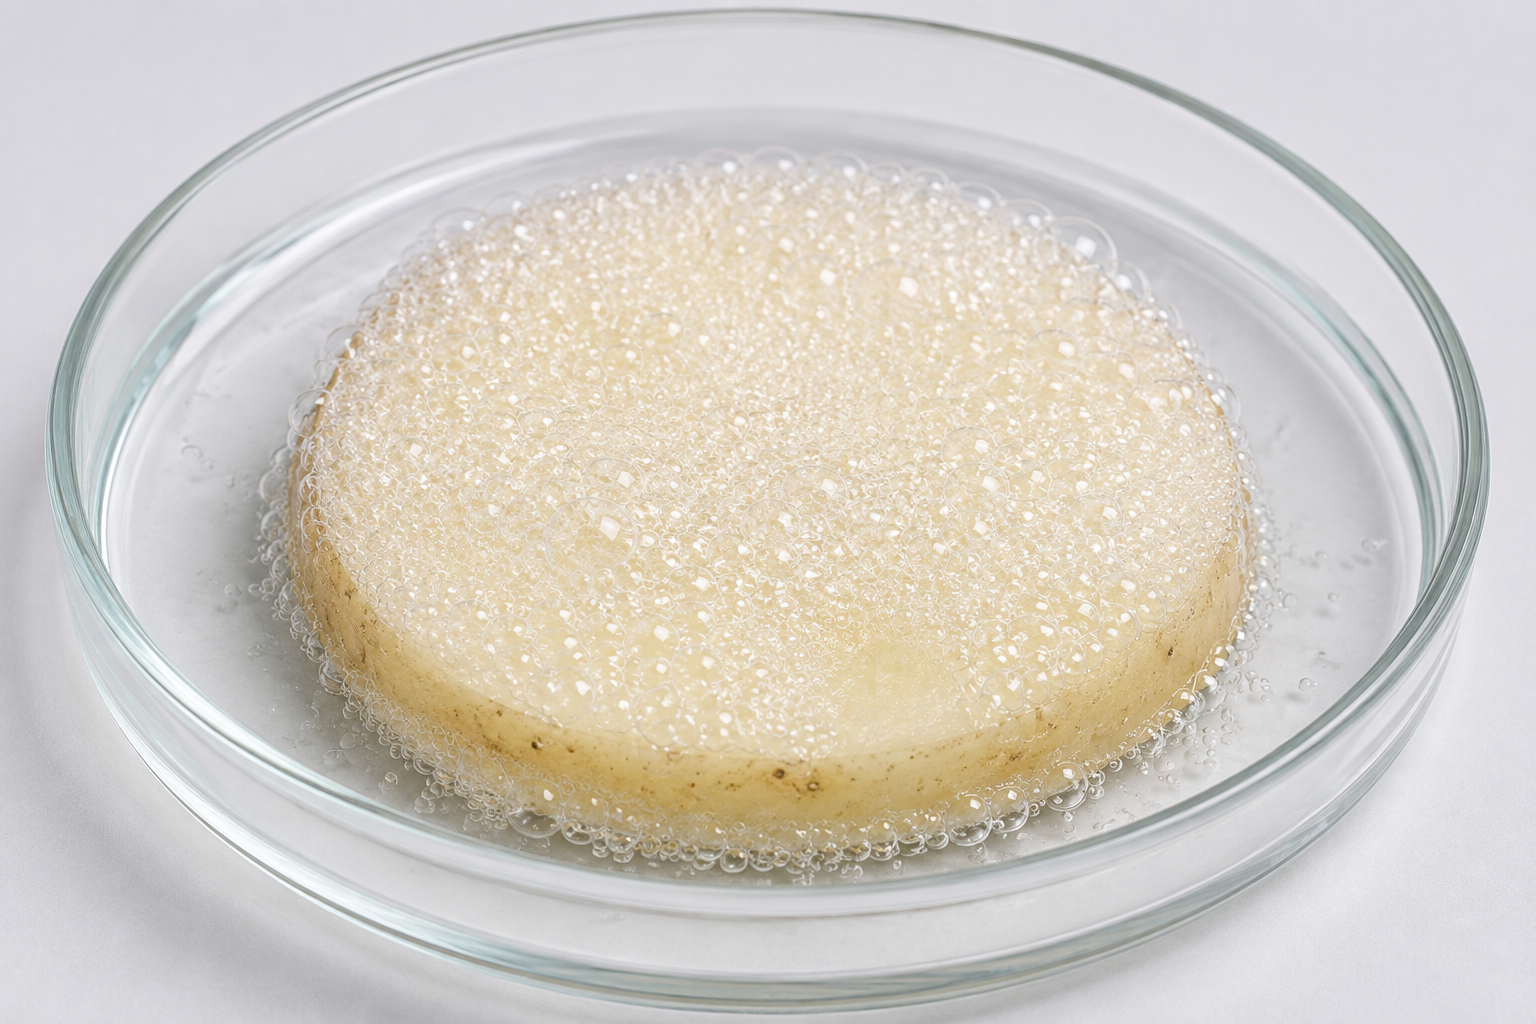
\includegraphics[width=0.5\linewidth]{images/book3/ai/b3-13-catalase-potato.png}

{\small ماء أكسجيني على بطاطا مقطوعة: الكاتالاز في \omterm{def:b1:cell-unit-of-life:cell}{الخلايا} يشطره إلى
ماء وأكسجين أربعين مليون مرة في الثانية لكل جزيء \omterm{def:b1:enzymes:enzyme}{إنزيم}، فيرغي
الأكسجين خارجًا.}
\end{omfigure}

\begin{proposition}[كيف يعمل الموقع الفعال]\label{prop:b1:enzymes:mechanisms}
يسرّع \omterm{def:b1:enzymes:enzyme}{الموقع الفعال} تفاعله بعدة وسائل في آن: فهو \emph{يربط ويوجّه}
الركائز حتى تلتقي الزمر المتفاعلة بالهندسة الصحيحة، فيستبدل بتصادم
نادر تصادمًا مؤكدًا؛ و\emph{يجهد} الركيزة نحو \omterm{prop:b1:enzymes:whatitdoes}{الحالة الانتقالية}
(\emph{التوافق المحرَّض}\index{التوافق المحرَّض}: إذ ينغلق \omterm{def:b1:enzymes:enzyme}{الإنزيم} حول
الركيزة، ويكون التوافق أحسن ما يكون مع \omterm{prop:b1:enzymes:whatitdoes}{الحالة الانتقالية})؛ وسلاسله
الجانبية تعمل عمل \emph{الحموض والأسس}، فتناول البروتونات للركيزة
وتأخذها منها في اللحظة المناسبة (والهيستيدين، وp$K_a$ له قرب 7، يفعل
هذا في \omterm{def:b1:enzymes:enzyme}{إنزيمات} كثيرة)؛ وبعضها يكوّن \emph{\omterm{def:b1:water-small-molecules:bonds}{رابطة تساهمية}} عابرة مع
الركيزة (بروتيازات السيرين)؛ وشوارده المعدنية تستقطب الروابط وتثبّت
الشحنات. والماء مستبعد إلى حد بعيد من الموقع، حتى تعمل الشحنات
\omterm{def:b1:water-small-molecules:water}{والروابط الهيدروجينية} بكامل قوتها.
\end{proposition}

\begin{example}[ثلاثة إنزيمات]\label{ex:b1:enzymes:three}
الليزوزيم، في الدموع وبياض البيض، يجهد حلقة سكرية من جدار البكتيريا
إلى شكل \omterm{prop:b1:enzymes:whatitdoes}{الحالة الانتقالية} ويقص السلسلة: بتسريع قدره $10^8$ ضعف.
والأنهيدراز الكربوني، في الكريات الحمراء، يحمل شاردة زنك تحوّل الماء
إلى هيدروكسيد مهيأ لمهاجمة $\mathrm{CO_2}$: أي مليون جزيء في
الثانية، وهو أسرع \omterm{def:b1:enzymes:enzyme}{إنزيم} بعد الكاتالاز. والكيموتربسين، في العصارة
البنكرياسية، يستعمل سيرينًا جعله هيستيدين فعالًا ليقص \omterm{def:b1:proteins:peptide}{البروتينات} بعد
البقايا العطرية: أي مئة في الثانية، مع وسيط تساهمي.
\end{example}

\section{حركية الإنزيمات}

\begin{definition}[المعدل الابتدائي والإشباع]\label{def:b1:enzymes:rate}
\emph{معدل}\index{معدل التفاعل} تفاعل إنزيمي $v$ هو كمية الناتج
المتكونة في واحدة الزمن (\unit{mol/s}، أو بوحدات إنزيمية:
\qty{1}{\micro mol/min}). ويُقاس \emph{معدلًا ابتدائيًا} $v_0$، قبل
أن تنفد الركيزة أو يتراكم الناتج. وعند تركيز إنزيمي ثابت يرتفع $v_0$
مع تركيز الركيزة $[S]$ ثم \emph{يتشبع} عند أقصى $V_{\max}$: إذ يكون
\omterm{def:b1:enzymes:enzyme}{الإنزيم} مشغولًا كله ولا يستطيع أن يسرع أكثر.
\end{definition}

\begin{theorem}[ميكايليس--منتن]\label{thm:b1:enzymes:mm}
\index{معادلة ميكايليس--منتن}\index{ثابت ميكايليس}
من أجل \omterm{def:b1:enzymes:enzyme}{إنزيم} $E$ يرتبط بركيزته ارتباطًا عكوسًا ويحوّلها،
\[
E + S \underset{k_{-1}}{\overset{k_1}{\rightleftharpoons}} ES
\overset{k_{\text{حفز}}}{\longrightarrow} E + P ,
\]
يكون المعدل الابتدائي عند تركيز ركيزة $[S]$
\[
v_0 = \frac{V_{\max}\,[S]}{K_m + [S]}, \qquad V_{\max} = k_{\text{حفز}}\,[E]_{\text{كلي}},
\qquad K_m = \frac{k_{-1} + k_{\text{حفز}}}{k_1} .
\]
و$K_m$، وهو \emph{\omterm{thm:b1:enzymes:mm}{ثابت ميكايليس}}، تركيزُ الركيزة الذي يكون المعدل
عنده نصف أقصاه، وهو يقيس كم ركيزة يحتاج \omterm{def:b1:enzymes:enzyme}{الإنزيم}؛ و$k_{\text{حفز}}$،
وهو \emph{عدد الدوران}\index{عدد الدوران}، عددُ جزيئات الركيزة التي
يحولها \omterm{def:b1:enzymes:enzyme}{إنزيم} واحد في الثانية حين يكون مشبعًا؛ والنسبة
$k_{\text{حفز}}/K_m$ هي \emph{المردود الحفزي}، وهو ثابت المعدل عند
ركيزة منخفضة، ويحده من فوق المعدلُ الذي تستطيع الركيزة أن تبلغ به
\omterm{def:b1:enzymes:enzyme}{الإنزيم} بالانتشار، وهو نحو
$10^8$--$10^9$ \unit{L.mol^{-1}.s^{-1}}.
\end{theorem}
\begin{proof}
افترض \emph{حالة مستقرة} يتكون فيها $ES$ بالسرعة التي يزول بها
(وهي صالحة بعد الميلي ثوان الأولى، ما دام $[S] \gg [E]$):
$k_1[E][S] = (k_{-1} + k_{\text{حفز}})[ES]$، فيكون $[E][S] = K_m[ES]$
حيث $K_m$ كما عُرِّف. والانحفاظ يعطي $[E] = [E]_{\text{كلي}} -
[ES]$؛ وبالتعويض، $([E]_{\text{كلي}} - [ES])[S] = K_m[ES]$، ومن ثم
$[ES] = [E]_{\text{كلي}}[S]/(K_m + [S])$. والمعدل هو
$v_0 = k_{\text{حفز}}[ES]$، وهذا يعطي الصيغة؛ وعند $[S] \gg K_m$
يكون $v_0 \to k_{\text{حفز}}[E]_{\text{كلي}} = V_{\max}$، وعند
$[S] = K_m$ يكون $v_0 = V_{\max}/2$.
\end{proof}

\begin{omfigure}
\begin{minipage}[b]{0.52\linewidth}\centering
\begin{tikzpicture}
\begin{axis}[
  width=\linewidth, height=5.6cm,
  axis x line=bottom, axis y line=left,
  xmin=0, xmax=22, ymin=0, ymax=1.12,
  xlabel={$[S]$ (\unit{mmol/L})}, ylabel={$v_0$ (\unit{\micro mol/min})},
  xlabel style={font=\small, at={(axis description cs:0.5,-0.14)}, anchor=north},
  ylabel style={font=\small},
  tick label style={font=\small}, xtick={0,5,10,15,20}, ytick={0,0.5,1},
  clip=false,
]
\addplot[very thick, omDef, domain=0:22, samples=100] {x/(2+x)};
\addplot[only marks, mark=*, mark size=1.6pt, omDef!70!black] coordinates {(0.5,0.2) (1,0.333) (2,0.5) (5,0.714) (10,0.833) (20,0.909)};
\draw[dashed, gray] (axis cs:0,1) -- (axis cs:22,1); \node[font=\scriptsize, anchor=south east] at (axis cs:22,1.0) {$V_{\max}$};
\draw[dashed, gray] (axis cs:0,0.5) -- (axis cs:2,0.5) -- (axis cs:2,0); \node[font=\scriptsize, anchor=north] at (axis cs:2,-0.02) {$K_m$};
\end{axis}
\end{tikzpicture}
\end{minipage}\hfill
\begin{minipage}[b]{0.46\linewidth}\centering
\begin{tikzpicture}
\begin{axis}[
  width=\linewidth, height=5.6cm,
  axis x line=middle, axis y line=left,
  xmin=-0.7, xmax=2.2, ymin=0, ymax=5.5,
  xlabel={$1/[S]$}, ylabel={$1/v_0$},
  xlabel style={font=\small, at={(axis description cs:0.5,-0.14)}, anchor=north},
  ylabel style={font=\small},
  tick label style={font=\small}, xtick={0,1,2}, ytick={1,3,5},
  clip=false,
]
\addplot[very thick, omDef, domain=-0.5:2.1, samples=10] {1 + 2*x};
\addplot[only marks, mark=*, mark size=1.6pt, omDef!70!black] coordinates {(2,5) (1,3) (0.5,2) (0.2,1.4) (0.1,1.2) (0.05,1.1)};
\node[font=\scriptsize, anchor=west, align=left] at (axis cs:0.05,4.6) {الميل $K_m/V_{\max}$};
\node[font=\scriptsize, anchor=west] at (axis cs:0.05,0.55) {$1/V_{\max}$};
\node[font=\scriptsize, anchor=south] at (axis cs:-0.5,0.1) {$-1/K_m$};
\end{axis}
\end{tikzpicture}
\end{minipage}

{\small إلى اليسار: زائدي ميكايليس--منتن من أجل $K_m = \qty{2}{mmol/L}$
و$V_{\max} = \qty{1}{\micro mol/min}$، مع النقاط الست المقيسة في
مسألة نهاية الأسبوع. وإلى اليمين: البيانات نفسها في مخطط
لاينويفر--بيرك، $1/v_0$ بدلالة $1/[S]$: وهو مستقيم تعطي تقاطعاته
$V_{\max}$ و$K_m$.}
\end{omfigure}

\begin{method}[قياس $K_m$ و$V_{\max}$]\label{met:b1:enzymes:lb}
\begin{enumerate}
  \item حضّر سلسلة من تراكيز الركيزة تمتد من $K_m/4$ إلى $10K_m$،
        بالتركيز الإنزيمي نفسه؛ وتابع الناتج (لونًا، أو امتصاصية، أو
        غازًا) في الدقيقة الأولى وخذ الميل $v_0$.
  \item ارسم $v_0$ بدلالة $[S]$: فيعطي الزائدي تقديرًا خشنًا
        للمقدار $V_{\max}$ (الهضبة) وللمقدار $K_m$ (التركيز عند
        نصفها).
  \item وللدقة، اقلب: $1/v_0 = (K_m/V_{\max})(1/[S]) +
        1/V_{\max}$
        (وهو \emph{لاينويفر--بيرك}). فتقاطع المستقيم مع محور $y$ هو
        $1/V_{\max}$، ومع محور $x$ هو $-1/K_m$، وميله
        $K_m/V_{\max}$.
  \item اقسم $V_{\max}$ على التركيز الإنزيمي لتحصل على
        $k_{\text{حفز}}$؛ واقسم على $K_m$ للمردود. وأعد التجربة مع
        مثبط لترى أي وسيط يغيره.
\end{enumerate}
\end{method}

\begin{omfigure}
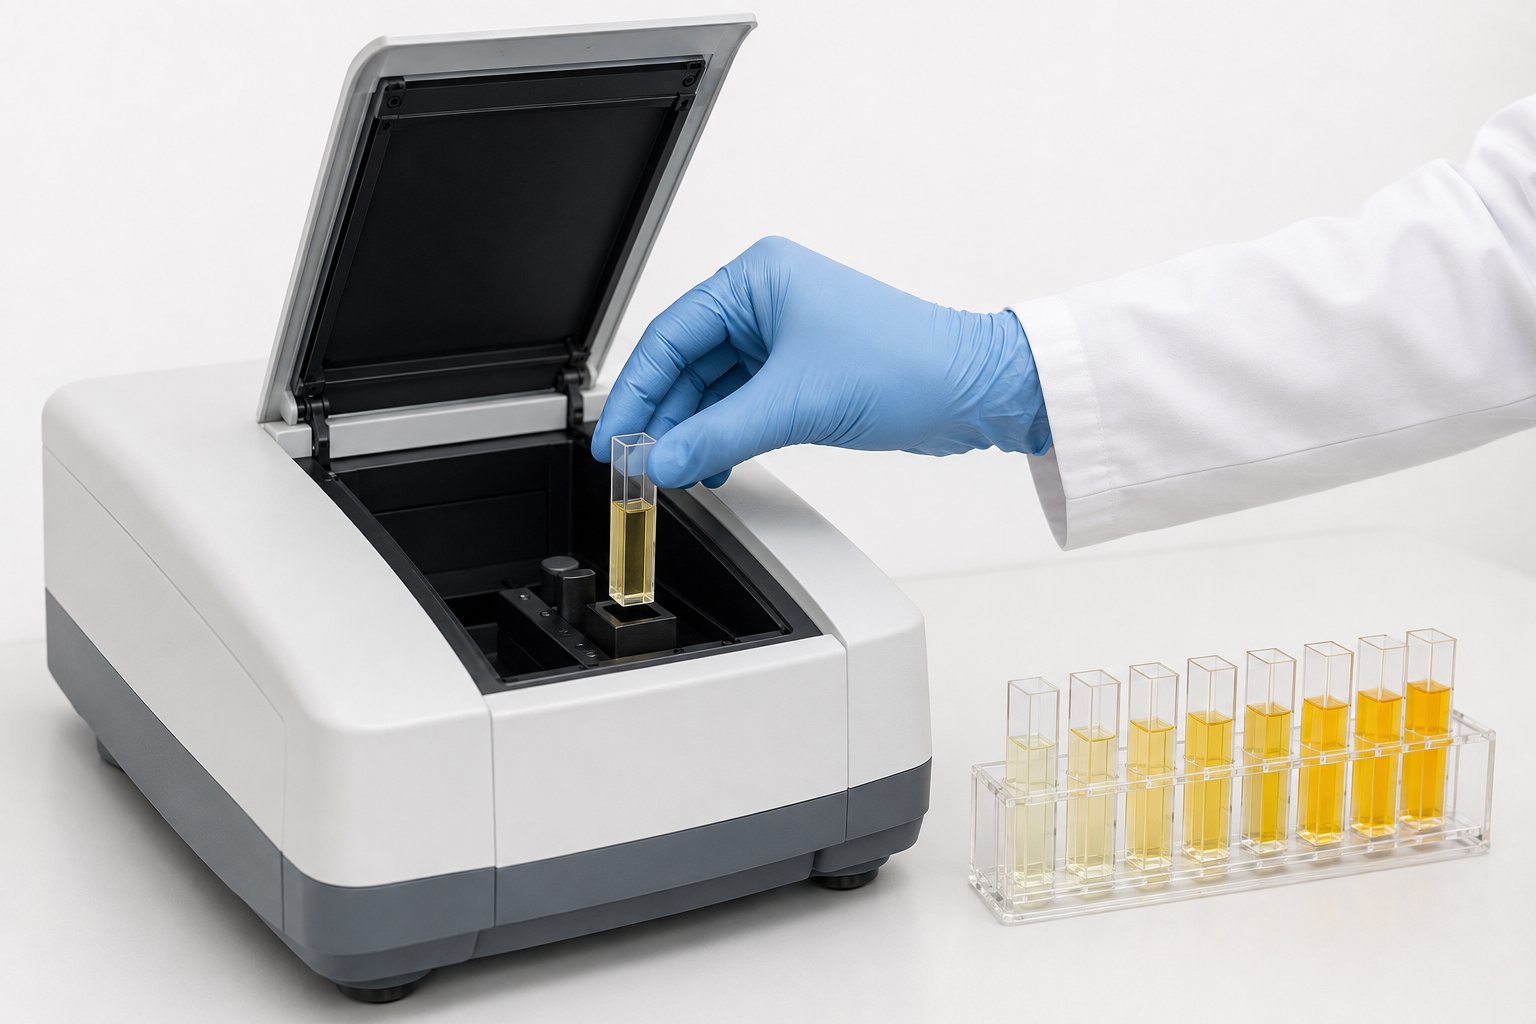
\includegraphics[width=0.5\linewidth]{images/book3/ai/b3-13-spectrophotometer-cuvette.png}

{\small مقايسة إنزيمية: الناتج يمتص الضوء، والمطياف الضوئي يسجل
ظهوره ثانيةً ثانية؛ والميل الابتدائي هو $v_0$.}
\end{omfigure}

\begin{example}[مقارنة إنزيمات]\label{ex:b1:enzymes:compare}
\begin{center}
\small
\begin{tabular}{lccc}
\hline
\omterm{def:b1:enzymes:enzyme}{الإنزيم} & $K_m$ (\unit{mol/L}) & $k_{\text{حفز}}$ (\unit{s^{-1}}) & $k_{\text{حفز}}/K_m$ (\unit{L.mol^{-1}.s^{-1}}) \\
\hline
الكاتالاز & \num{2.5e-2} & \num{4e7} & \num{1.6e9} \\
الأنهيدراز الكربوني & \num{1.2e-2} & \num{1e6} & \num{8e7} \\
الكيموتربسين & \num{1.5e-2} & 100 & \num{7e3} \\
الليزوزيم & \num{6e-6} & 0.5 & \num{8e4} \\
بوليميراز \omterm{def:b1:nucleic-acids:chain}{DNA} & \num{1e-5} & 15 & \num{1.5e6} \\
\hline
\end{tabular}
\end{center}
الكاتالاز والأنهيدراز الكربوني يعملان عند حد الانتشار: فكل تصادم مع
الركيزة منتج. والكيموتربسين بطيء لكنه يحتاج أن يكون كذلك --- فهو يقص
\omterm{def:b1:proteins:peptide}{رابطة ببتيدية}، وهي عمل أصعب بكثير من شطر ماء أكسجيني.
\end{example}

\section{التثبيط}

\begin{definition}[المثبطات]\label{def:b1:enzymes:inhibitors}
\emph{المثبط}\index{مثبط الإنزيم} يخفض معدل \omterm{def:b1:enzymes:enzyme}{إنزيم}. والمثبطات
\emph{اللاعكوسة} ترتبط تساهميًا وتتلف نشاط \omterm{def:b1:enzymes:enzyme}{الإنزيم} إلى الأبد (العوامل
العصبية على إستيراز الأستيل كولين، والبنسلين على \omterm{def:b1:enzymes:enzyme}{الإنزيم} الذي يشابك
جدار البكتيريا، والأسبرين على \omterm{def:b1:enzymes:enzyme}{الإنزيم} الذي يصنع البروستاغلاندينات).
أما المثبطات \emph{العكوسة} فترتبط بروابط ضعيفة ويمكن غسلها؛ وبحسب
موضع ارتباطها:
\begin{itemize}
  \item \emph{تنافسي}\index{التثبيط التنافسي}: يشبه المثبط الركيزة
        ويشغل \omterm{def:b1:enzymes:enzyme}{الموقع الفعال}؛ فيرفع $K_m$ الظاهري (بالعامل
        $1 + [I]/K_i$) ويترك $V_{\max}$ على حاله --- فركيزة كافية
        تزيحه؛
  \item \emph{غير تنافسي}: يرتبط المثبط في موضع آخر ويفسد الحفز سواء
        أكانت الركيزة مرتبطة أم لا؛ فيخفض $V_{\max}$ ويترك $K_m$ على
        حاله --- ولا يتغلب عليه أي قدر من الركيزة؛
  \item \emph{مضاد التنافس}: لا يرتبط المثبط إلا بالمعقد $ES$؛
        فيهبط $V_{\max}$ و$K_m$ معًا.
\end{itemize}
و$K_i$، وهو ثابت انفكاك المثبط، يقيس قوته: فكلما انخفض كان أقوى.
\end{definition}

\begin{omfigure}
\begin{tikzpicture}
\begin{axis}[
  width=0.8\linewidth, height=6.0cm,
  axis x line=middle, axis y line=left,
  xmin=-0.8, xmax=2.2, ymin=0, ymax=10.5,
  xlabel={$1/[S]$}, ylabel={$1/v_0$},
  xlabel style={font=\small, at={(axis description cs:0.5,-0.1)}, anchor=north},
  ylabel style={font=\small},
  tick label style={font=\small}, xtick={0,1,2}, ytick={2,4,6,8,10},
  legend style={font=\small, at={(0.03,0.97)}, anchor=north west, draw=none},
  clip=false,
]
\addplot[very thick, omDef, domain=-0.5:2.1, samples=10] {1 + 2*x};
\addlegendentry{بلا مثبط}
\addplot[very thick, omThm, domain=-0.25:2.1, samples=10] {1 + 4*x};
\addlegendentry{تنافسي: $1/V_{\max}$ نفسه، وأشد ميلًا}
\addplot[very thick, omProp, domain=-0.5:2.1, samples=10] {2 + 4*x};
\addlegendentry{غير تنافسي: $-1/K_m$ نفسه، وأعلى}
\end{axis}
\end{tikzpicture}

{\small مخططا لاينويفر--بيرك مع المثبطين الشائعين. \omterm{def:b1:enzymes:inhibitors}{المثبط} \omterm{def:b1:enzymes:inhibitors}{التنافسي}
يدير المستقيم حول تقاطع $y$ ($V_{\max}$ على حاله، و$K_m$ مرتفع)؛
وغير \omterm{def:b1:enzymes:inhibitors}{التنافسي} يديره حول تقاطع $x$ ($K_m$ على حاله، و$V_{\max}$
منخفض).}
\end{omfigure}

\begin{example}[المنافسة دواءً]\label{ex:b1:enzymes:medicine}
الميثانول غير مؤذٍ حتى تحوله نازعة هيدروجين الكحول في الكبد إلى
فورمألدهيد \omterm{def:b1:water-small-molecules:ph}{وحمض} النمل، وهما يعميان ويقتلان. والعلاج هو الإيثانول:
ركيزة منافسة له $K_m$ أدنى، تُبقي \omterm{def:b1:enzymes:enzyme}{الإنزيم} مشغولًا بينما يُطرح
الميثانول دون تغير. والستاتينات مثبطات تنافسية، تشبه \omterm{prop:b1:enzymes:whatitdoes}{الحالة
الانتقالية}، \omterm{def:b1:enzymes:enzyme}{للإنزيم} الذي يلزم الكربون بطريق \omterm{def:b1:lipids:amphiphilic}{الكولستيرول}؛ والسلفوناميدات
تشبه ركيزة \omterm{def:b1:enzymes:enzyme}{إنزيم} بكتيري يصنع الفولات، وهو ما لا يصنعه الإنسان فلا
يفتقده.
\end{example}

\section{التنظيم}

\begin{definition}[الإنزيمات الألوستيرية]\label{def:b1:enzymes:allosteric}
\emph{للإنزيم الألوستيري}\index{إنزيم ألوستيري} عدة وحدات، وله، فضلًا
عن مواقعه الفعالة، \emph{مواقع تنظيمية} ترتبط بها المؤثرات:
\emph{فالمنشطات} تزيحه نحو تشكيله الفعال، و\emph{المثبطات} نحو غير
الفعال. ومعدله بدلالة $[S]$ سيني لا زائدي (بتعاون بين المواقع
الفعالة، كما عند الهيموغلوبين، \cref{ch:b1:proteins})، فيغير تغيرٌ
صغير في الركيزة قرب الجزء الحاد المعدلَ تغييرًا كبيرًا؛ والمؤثرات
تزيح المنحني جانبًا (فتغير تركيز الركيزة اللازم) أو صعودًا وهبوطًا
(فتغير المعدل الأقصى). \omterm{def:b1:enzymes:enzyme}{والإنزيمات} \omterm{def:b1:proteins:allostery}{الألوستيرية} تقف عند نقاط تفرع
الاستقلاب، والمؤثرات هي نواتج السبيل نفسها وإشارات طاقة \omterm{def:b1:cell-unit-of-life:cell}{الخلية} (\omterm{def:b1:water-small-molecules:atp}{ATP}،
وADP، وAMP).
\end{definition}

\begin{omfigure}
\begin{tikzpicture}
\begin{axis}[
  width=0.86\linewidth, height=6.0cm,
  axis x line=bottom, axis y line=left,
  xmin=0, xmax=10, ymin=0, ymax=1.1,
  xlabel={$[S]$ (نسبي)}, ylabel={$v_0/V_{\max}$},
  xlabel style={font=\small, at={(axis description cs:0.5,-0.12)}, anchor=north},
  ylabel style={font=\small},
  tick label style={font=\small}, xtick={0,2,4,6,8,10}, ytick={0,0.5,1},
  legend style={font=\small, at={(0.5,-0.22)}, anchor=north, draw=none, legend columns=2, /tikz/every even column/.append style={column sep=0.4cm}},
  clip=false,
]
\addplot[very thick, omDef, domain=0:10, samples=100] {x^3/(3^3+x^3)};
\addlegendentry{إنزيم ألوستيري وحده ($n = 3$)}
\addplot[very thick, omExo, domain=0:10, samples=100] {x^3/(1.8^3+x^3)};
\addlegendentry{مع منشط: المنحني ينزاح يسارًا}
\addplot[very thick, omThm, domain=0:10, samples=100] {x^3/(5.5^3+x^3)};
\addlegendentry{مع مثبط: المنحني ينزاح يمينًا}
\addplot[thick, dashed, gray, domain=0:10, samples=100] {x/(3+x)};
\addlegendentry{ميكايليس--منتن، للمقارنة}
\draw[dashed, gray] (axis cs:3,0) -- (axis cs:3,0.5);
\end{axis}
\end{tikzpicture}

{\small \omterm{def:b1:enzymes:allosteric}{إنزيم ألوستيري}. المنحني السيني يجعل المعدل حساسًا للركيزة قرب
المنتصف؛ والمنشط يزيحه يسارًا (فيصير أنشط عند $[S]$ معطى)، \omterm{def:b1:enzymes:inhibitors}{والمثبط}
يمينًا. وقرب $[S] = 3$ يستطيع المعدل أن ينساح من عُشر الأقصى إلى تسعة
أعشاره.}
\end{omfigure}

\begin{proposition}[أربع طرق تتحكم بها الخلية في إنزيم]\label{prop:b1:enzymes:control}
\begin{enumerate}
  \item \emph{التثبيط الراجع}\index{التثبيط الراجع}: يكون الناتج
        النهائي لسبيل مثبطًا \omterm{def:b1:proteins:allostery}{ألوستيريًا} لأول \omterm{def:b1:enzymes:enzyme}{إنزيم} ملتزم فيه، فلا
        يجري السبيل إلا بقدر ما يُستهلك الناتج (الإيزولوسين على نازعة
        أمين الثريونين؛ \omterm{def:b1:water-small-molecules:atp}{وATP} على فسفوفركتوكيناز،
        \cref{ch:b1:respiration-fermentation}). وزمن الاستجابة:
        أجزاء من الألف من الثانية.
  \item \emph{التعديل التساهمي}\index{التعديل التساهمي}: يعلّق كيناز
        فوسفاتًا على سيرين أو ثريونين أو تيروزين في \omterm{def:b1:enzymes:enzyme}{الإنزيم}، وينزعه
        فوسفاتاز، وتختلف الصورتان في النشاط (فسفوريلاز \omterm{def:b1:carbohydrates:polysaccharide}{الغليكوجين}
        يُشغَّل بالفسفرة، وسنتاز \omterm{def:b1:carbohydrates:polysaccharide}{الغليكوجين} يُطفأ بها، بالإشارة
        الهرمونية نفسها). وذلك في ثوان إلى دقائق؛ وهو عكوس؛ ويمكن
        تضخيمه في شلالات.
  \item \emph{التنشيط \omterm{prop:b1:water-small-molecules:families}{بالحلمهة} البروتينية}: تُصنع بعض \omterm{def:b1:enzymes:enzyme}{الإنزيمات}
        طلائع خاملة (\emph{طلائع \omterm{def:b1:enzymes:enzyme}{إنزيمات}}: طليعة التربسين، وطليعة
        الببسين، وعوامل التخثر) وتُشغَّل بقص ببتيد منها، مرة واحدة
        وإلى الأبد، حيث تُراد ومتى تُراد.
  \item \emph{الكمية}: تصنع \omterm{def:b1:cell-unit-of-life:cell}{الخلية} من \omterm{def:b1:enzymes:enzyme}{الإنزيم} أكثر أو أقل بالتحكم في
        مورّثته (\cref{ch:b1:expression-control}) وتهدمه أسرع أو
        أبطأ. وذلك في دقائق إلى ساعات.
\end{enumerate}
\end{proposition}

\begin{example}[الإنزيمات المتماثلة]\label{ex:b1:enzymes:isoenzymes}
نازعة هيدروجين اللاكتات موجودة في خمس صور، وهي رباعيات من نوعي وحدات
بكل التراكيب؛ وصورة القلب لها $K_m$ منخفض للاكتات ويثبطها البيروفات
(فهي تؤكسد اللاكتات لتغذي دورة كريبس)، وصورة العضلة لها $V_{\max}$
مرتفع وتحتمل البيروفات (فهي تصنع اللاكتات في عدو سريع). ونمط الصور في
الدم يكشف أي \omterm{def:b1:mammal-organization:organ}{عضو} قد تضرر --- فالنوبة القلبية تحرر صورة القلب.
\end{example}

\section{الحرارة وpH}

\begin{proposition}[الإنزيمات ومحيطها]\label{prop:b1:enzymes:environment}
يتضاعف \omterm{def:b1:enzymes:rate}{معدل التفاعل} الإنزيمي تقريبًا كل \qty{10}{\celsius}
($Q_{10} \approx 2$) كلما حملت الطاقة الحرارية جزيئات أكثر فوق
الحاجز، إلى أن يبدأ \omterm{def:b1:enzymes:enzyme}{الإنزيم} بالانفكاك
(\qtyrange{40}{60}{\celsius} عند معظمها؛ و\qty{100}{\celsius} عند
\omterm{def:b1:enzymes:enzyme}{إنزيمات} بكتيريا الينابيع الحارة) فينهار المعدل. ولكل \omterm{def:b1:enzymes:enzyme}{إنزيم}
\emph{pH مثلى}، تكون عندها برتنة بقاياه الحفازة وبرتنة ركيزته
صحيحة: فالببسين، في المعدة، قرب pH 2؛ والتربسين، في المعي، قرب 8؛
ومعظم \omterm{def:b1:enzymes:enzyme}{الإنزيمات} داخل الخلوية قرب 7. وبعيدًا عن المثلى يهبط المعدل،
وبعيدًا جدًا يُمسخ \omterm{def:b1:proteins:peptide}{البروتين}. فالحرارة وpH تعملان في \omterm{def:b1:proteins:peptide}{البروتين}؛ \omterm{def:b1:cell-unit-of-life:cell}{والخلية}
تبقيهما في المدى الذي تعمل فيه إنزيماتها الألف كلها.
\end{proposition}

\begin{example}[حمى وينبوع حار]\label{ex:b1:enzymes:fever}
حمى قدرها \qty{40}{\celsius} تسرّع كل تفاعل في الجسم بمقدار الربع
وتبدأ بفك أهش \omterm{def:b1:proteins:peptide}{البروتينات}؛ وعند \qty{42}{\celsius} تفشل \omterm{def:b1:proteins:peptide}{بروتينات}
الدماغ. وبوليميراز \omterm{def:b1:nucleic-acids:chain}{DNA} عند بكتيريا من ينبوع عند \qty{75}{\celsius}
ينجو من \qty{95}{\celsius}، ولهذا يمكن تدويره عبر صهر \omterm{def:b1:nucleic-acids:chain}{DNA} آلاف
المرات وصار \omterm{def:b1:enzymes:enzyme}{إنزيم} تفاعل البوليميراز المتسلسل (كتاب السنة الثالثة):
فالثبات الحراري خاصية للتسلسل لا للكيمياء المحفوزة.
\end{example}

\section{تمارين}

\begin{exercise}[$\star$]\label{exo:b1:enzymes:1}
ما الذي يغيره \omterm{def:b1:enzymes:enzyme}{الإنزيم} في تفاعل، وما الذي يتركه على حاله؟ وضّح
بمنحني الطاقة.
\end{exercise}

\begin{exercise}[$\star$]\label{exo:b1:enzymes:2}
عرّف $K_m$ و$V_{\max}$ و$k_{\text{حفز}}$ و$k_{\text{حفز}}/K_m$، مع
الوحدات.
\end{exercise}

\begin{exercise}[$\star$]\label{exo:b1:enzymes:3}
من شكل لاينويفر--بيرك للمثبطات، اقرأ $V_{\max}$ و$K_m$ عند \omterm{def:b1:enzymes:enzyme}{الإنزيم}
غير المثبَّط وعند كل مثبط.
\end{exercise}

\begin{exercise}[$\star$]\label{exo:b1:enzymes:4}
سمِّ الطرق الأربع التي تنظم بها \omterm{def:b1:cell-unit-of-life:cell}{الخلية} نشاط \omterm{def:b1:enzymes:enzyme}{إنزيم} وأعطِ المقياس
الزمني لكل منها.
\end{exercise}

\begin{exercise}[$\star\star$]\label{exo:b1:enzymes:5}
\omterm{def:b1:enzymes:enzyme}{إنزيم} له $K_m = \qty{0.1}{mmol/L}$ و$V_{\max} =
\qty{50}{\micro mol/min}$.
احسب $v_0$ عند $[S] = 0.02$ و$0.1$ و$1$ و\qty{10}{mmol/L}. وعند أي
$[S]$ يكون $v_0 = 0.9\,V_{\max}$؟
\end{exercise}

\begin{exercise}[$\star\star$]\label{exo:b1:enzymes:6}
خفض $E_a$ بمقدار \qty{20}{kJ/mol} عند \qty{37}{\celsius} يضرب المعدل
في أي عامل؟ وبكم يجب أن تهبط $E_a$ لكسب عامل قدره $10^{10}$؟
\end{exercise}

\begin{exercise}[$\star\star$]\label{exo:b1:enzymes:7}
$\qty{2}{pmol}$ من الأنهيدراز الكربوني في \qty{1}{mL} تعطي
$V_{\max} = \qty{120}{mmol/L}$ في الدقيقة. احسب $k_{\text{حفز}}$،
ثم المردود مع $K_m = \qty{12}{mmol/L}$. وقارن مع حد الانتشار.
\end{exercise}

\begin{exercise}[$\star\star$]\label{exo:b1:enzymes:8}
مثبط \omterm{def:b1:enzymes:inhibitors}{تنافسي} عند \qty{2}{mmol/L} يضاعف $K_m$ الظاهري. احسب $K_i$. وأي
تركيز ركيزة يعيد المعدل إلى \qty{90}{\%} من $V_{\max}$ مع \omterm{def:b1:enzymes:inhibitors}{المثبط}
وبدونه، إذا كان $K_m = \qty{1}{mmol/L}$؟
\end{exercise}

\begin{exercise}[$\star\star$]\label{exo:b1:enzymes:9}
فسّر لماذا يعمل \omterm{prop:b1:enzymes:control}{التثبيط الراجع} على أول خطوة ملتزمة في سبيل لا على
الأخيرة، ولماذا كان \omterm{def:b1:enzymes:inhibitors}{المثبط} عادة الناتج النهائي لا وسيطًا.
\end{exercise}

\begin{exercise}[$\star\star\star$]\label{exo:b1:enzymes:10}
تُنشَّط طليعة التربسين في المعي لا في البنكرياس الذي يصنعها؛ وكسر
صغير منها ينشَّط باكرًا يتلف البنكرياس. فسّر منطق طلائع \omterm{def:b1:enzymes:enzyme}{الإنزيمات}،
ودور \omterm{def:b1:enzymes:enzyme}{الإنزيم} الذي ينشّط طليعة التربسين، ولماذا يصنع البنكرياس أيضًا
مثبطًا للتربسين.
\end{exercise}

\begin{exercise}[$\star\star\star$]\label{exo:b1:enzymes:11}
\omterm{def:b1:enzymes:allosteric}{إنزيم ألوستيري} عند $n = 3$ ونصف إشباع عند $[S]_{0.5}
= 3$ يزيح مثبطٌ
منحنيَه إلى $[S]_{0.5} = 5.5$. احسب المعدل عند $[S] = 3$ مع \omterm{def:b1:enzymes:inhibitors}{المثبط}
وبدونه، وقارن بالتغير الذي كان مثبط \omterm{def:b1:enzymes:inhibitors}{تنافسي} بالإزاحة نفسها في $K_m$
ليحدثه على \omterm{def:b1:enzymes:enzyme}{إنزيم} ميكايليس--منتن. فماذا تضيف \omterm{def:b1:proteins:allostery}{التعاونية} إلى التنظيم؟
\end{exercise}

\begin{exercise}[$\star\star\star$]\label{exo:b1:enzymes:12}
«\omterm{def:b1:enzymes:enzyme}{الإنزيم} حفاز قيل له ماذا يفعل.» ناقش في فقرة: الحفز في مقابل
النوعية، والتنظيم بوصفه المعلومة المضافة، وكلفة \omterm{def:b1:enzymes:enzyme}{إنزيم} منظَّم قياسًا
إلى حفاز مجرد.
\end{exercise}

\section{مسألة: إنزيم مقيس}

\begin{problem}[{مسألة نهاية الأسبوع --- إستيراز يُقايَس عند ستة
تراكيز ركيزة، وحده ومع مثبطين، وتُستخرج ثوابته ويُتنبأ بسلوكه في
\omterm{def:b1:cell-unit-of-life:cell}{الخلية}، وصولًا إلى $K_m$ و$V_{\max}$ و$K_i$ له}]
\label{pb:b1:enzymes:1}
يُقايَس إستيراز في \qty{1.0}{mL} عند \qty{25}{\celsius} وpH 7.5، مع
\qty{10}{nmol/L} من \omterm{def:b1:enzymes:enzyme}{الإنزيم}. والمعدلات الابتدائية
(\unit{\micro mol/min}) عند ستة تراكيز ركيزة، وحدها وبوجود
\qty{1.0}{mmol/L} من \omterm{def:b1:enzymes:inhibitors}{المثبط} I أو \qty{1.0}{mmol/L} من \omterm{def:b1:enzymes:inhibitors}{المثبط} J:

\begin{center}
\small
\begin{tabular}{lcccccc}
\hline
$[S]$ (\unit{mmol/L}) & 0.5 & 1 & 2 & 5 & 10 & 20 \\
\hline
$v_0$، بلا مثبط & 0.200 & 0.333 & 0.500 & 0.714 & 0.833 & 0.909 \\
$v_0$، مع I & 0.111 & 0.200 & 0.333 & 0.556 & 0.714 & 0.833 \\
$v_0$، مع J & 0.100 & 0.167 & 0.250 & 0.357 & 0.417 & 0.455 \\
\hline
\end{tabular}
\end{center}

\medskip
\noindent\textbf{الجزء الأول --- \omterm{def:b1:enzymes:enzyme}{الإنزيم} وحده.}
\begin{enumerate}
  \item احسب $1/[S]$ و$1/v_0$ للنقاط الست بلا مثبط.
  \item بيّن أن النقاط تقع على مستقيم وأوجد ميله وتقاطعه.
  \item استنتج $V_{\max}$ و$K_m$.
  \item تحقق \omterm{thm:b1:enzymes:mm}{بمعادلة ميكايليس--منتن} عند $[S] =
        \qty{5}{mmol/L}$.
  \item احسب كمية \omterm{def:b1:enzymes:enzyme}{الإنزيم} في المقايسة (بالمول) و$k_{\text{حفز}}$
        بوحدة \unit{s^{-1}}.
  \item احسب $k_{\text{حفز}}/K_m$ وقارنه بحد الانتشار.
  \item عند أي تركيز ركيزة يعمل \omterm{def:b1:enzymes:enzyme}{الإنزيم} عند \qty{95}{\%} من
        $V_{\max}$؟
\end{enumerate}

\medskip
\noindent\textbf{الجزء الثاني --- \omterm{def:b1:enzymes:inhibitors}{المثبط} I.}
\begin{enumerate}[resume]
  \item احسب $1/v_0$ للنقاط الست مع I وأوجد ميل مستقيمها وتقاطعه.
  \item استنتج $V_{\max}$ و$K_m$ الظاهريين مع I.
  \item أي وسيط تغير؟ صنّف \omterm{def:b1:enzymes:inhibitors}{المثبط}.
  \item احسب $K_i$ من $K_m^{\text{ظاهري}} = K_m(1 + [I]/K_i)$.
  \item عند $[S] = \qty{2}{mmol/L}$، أي تركيز من I ينصّف المعدل؟
        وعند $[S] = \qty{20}{mmol/L}$؟
  \item اقترح ما يمكن أن يكونه I بنيويًا، وأين يرتبط.
\end{enumerate}

\medskip
\noindent\textbf{الجزء الثالث --- \omterm{def:b1:enzymes:inhibitors}{المثبط} J.}
\begin{enumerate}[resume]
  \item احسب ميل المستقيم مع J وتقاطعه واستنتج $V_{\max}$ و$K_m$
        الظاهريين.
  \item صنّف J واحسب $K_i$ له من $V_{\max}^{\text{ظاهري}} =
        V_{\max}/(1 + [J]/K_i)$.
  \item فسّر لماذا لا يستطيع رفع الركيزة أن يتغلب على J.
  \item مضاعفة تركيز \omterm{def:b1:enzymes:enzyme}{الإنزيم} بوجود J تفعل ماذا بالمعدل؟ وبوجود I؟
\end{enumerate}

\medskip
\noindent\textbf{الجزء الرابع --- في \omterm{def:b1:cell-unit-of-life:cell}{الخلية}.}
تبقي \omterm{def:b1:cell-unit-of-life:cell}{الخلية} الركيزة عند \qty{0.5}{mmol/L} \omterm{def:b1:enzymes:enzyme}{والإنزيم} عند
\qty{10}{nmol/L} في حجم قدره \qty{1000}{\micro m^3}، عند
\qty{37}{\celsius}، مع $Q_{10} = 2$.
\begin{enumerate}[resume]
  \item احسب المعدل في \omterm{def:b1:cell-unit-of-life:cell}{الخلية} (بجزيئات الناتج في الثانية في \omterm{def:b1:cell-unit-of-life:cell}{الخلية}
        كلها).
  \item يُطلب الناتج بمعدل \qty{3e6}{} جزيء في الثانية. فبأي عامل
        يجب أن ترفع \omterm{def:b1:cell-unit-of-life:cell}{الخلية} المعدل، وسمِّ طريقتين تستطيعهما.
  \item الناتج مثبط \omterm{def:b1:enzymes:inhibitors}{تنافسي} \omterm{def:b1:enzymes:enzyme}{للإنزيم} عند $K_i = \qty{0.2}{mmol/L}$،
        وهو يتراكم إلى \qty{0.4}{mmol/L}. احسب المعدل عندئذ، وعلّق
        على ما يحققه ذلك.
  \item يُفسفَر \omterm{def:b1:enzymes:enzyme}{الإنزيم} بكيناز، فيخفض $K_m$ له إلى \qty{0.4}{mmol/L}.
        احسب المعدل عند \qty{0.5}{mmol/L} من الركيزة قبل ذلك وبعده.
  \item pH المثلى \omterm{def:b1:enzymes:enzyme}{للإنزيم} 7.5 وينتصف نشاطه عند pH 6.5. \omterm{def:b1:eukaryotic-cell:endomembrane}{والجسيم الحال}
        عند pH 5. تنبأ نوعيًا بنشاطه هناك وفسّر بدلالة البقايا
        القابلة للتشرد.
  \item طفرة تستبدل بالهيستيدين في \omterm{def:b1:enzymes:enzyme}{الموقع الفعال} ألانينًا. تنبأ
        بالأثر في $K_m$ وفي $k_{\text{حفز}}$، مع سبب لكل منهما.
  \item فسّر لماذا تبقي \omterm{def:b1:cell-unit-of-life:cell}{الخلية} الركيزة قرب $K_m$ لا فوقه بكثير.
  \item اذكر النتيجة: $K_m$ و$V_{\max}$ و$k_{\text{حفز}}$ للإستيراز،
        ونوع كل مثبط و$K_i$ له.
\end{enumerate}
\end{problem}
